\section[Smart grid overview]{\Gls{sg} overview}
%\label{sec:example:sg}

\begin{figure*}[ht]
	\centering
    \subfloat[Electricity flow 1] {
		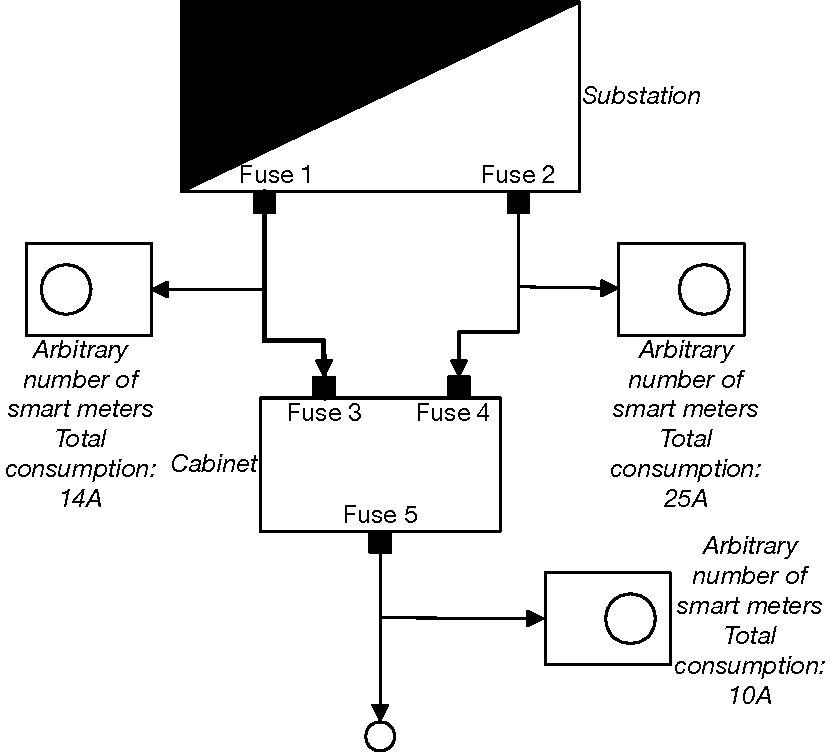
\includegraphics[width=.45\linewidth]{img/chapt-example/duc/Topology1}
		\label{fig:example:sg-overview:topo1}
	}
	\hfill
	\subfloat[Electricity flow 2] {
		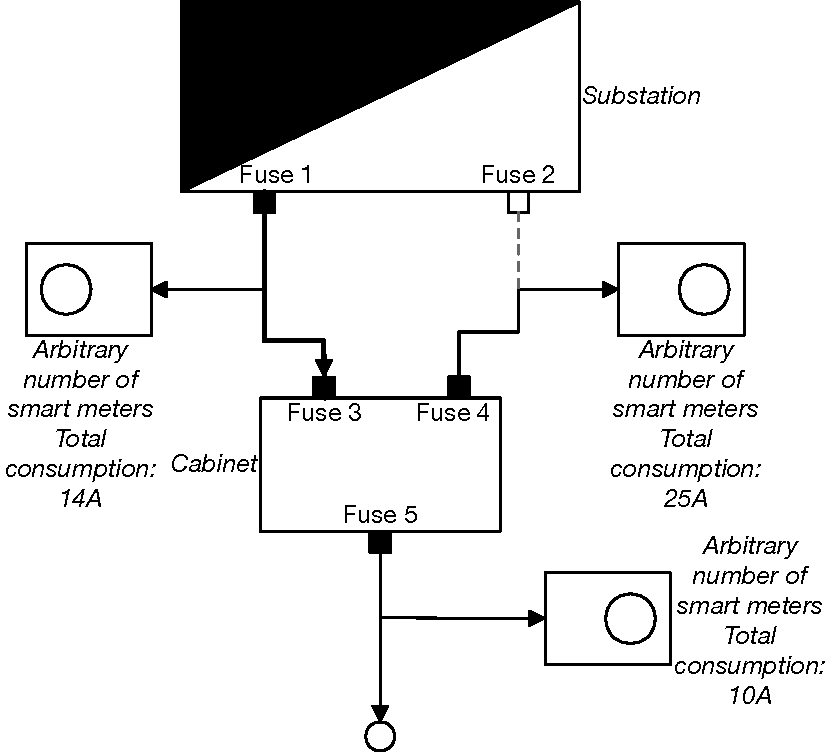
\includegraphics[width=.45\linewidth]{img/chapt-example/duc/Topology2}
		\label{fig:example:sg-overview:topo2}
	}
	\caption{Two different electric flows for a same grid topology}
	\label{fig:example:sg-overview:topo}
\end{figure*}



The National Institute of Standards and Technology (NIST) defines a \gls{sg} as ``a planned nationwide network that uses information technology to deliver electricity efficiently, reliably, and securely"\footnote{\url{https://www.nist.gov/engineering-laboratory/smart-grid/smart-grid-beginners-guide}}.
Conceptually, a \gls{sg} is composed of different entities, like smart meters, cabinets (connection points of cables) and power substations.
These entities are connected, forming a network, and able to exchange information using different technologies~\cite{DBLP:conf/smartgridcomm/0001FKTPTR14, DBLP:conf/sac/0001MFRKT16}.

The network is the connection linking the \gls{sg} entities by means of physical cables. 
Every cable has a maximum load depending on its diameter and the used material.
\Cref{fig:example:sg-overview:topo} depicts an example of such a network. 
This network is composed of one substation, one cabinet, and an arbitrary number of smart meters.
Every cable has two fuses (to connect or disconnect the cable), one at each endpoint.
By opening or closing fuses, one can influence the electricity flow through the network.
\Cref{fig:example:sg-overview:topo1} and~\ref{fig:example:sg-overview:topo2} show two possible electricity flows over the same physical network. 
We depict closed fuses in black and the direction of the electricity flow using black arrows.

Smart meters continuously measure electricity consumption and periodically report it to a central data centre.
Based on this information, together with the grid topology, the electric load of cables can be computed.
If the reader wants to go more into the details of this computation, we invite him or her to read~\cite{DBLP:conf/sac/0001MFRKT16}.
The flow has a big impact on the load cables.
In \autoref{fig:example:sg-overview:topo}, we depict two different flows for the same grid topology.
In both cases, the measured electric consumption are equal.
However, in \Cref{fig:example:sg-overview:topo1} the load on the left cable (thick line) equals $\frac{14 + 25 + 10}{2} = 24.5$ whereas it equals $14+25+10=49$ in \Cref{fig:example:sg-overview:topo2}.

The central system monitors electric loads to avoid any overload in the network, implementing the \gls{adptSyst} vision.
In the remaining part of this document, we refer to this goal as the "\textit{no overload}" policy.
They have two \gls{action} points: either on the production side or the consumption side.
They can reduce or increase the production by (dis)connecting production unit or the consumption by modifying the maximum permitted consumption.
We called these actions: \textit{reduce production}, \textit{increase production}, \textit{reduce amps limit} and \textit{increase amps limit}.
However, as all adaptive systems, \gls{sg}s are prone to failures~\cite{DBLP:conf/smartgridsec/0001FKNT14}.
In case of a failure, an engineer could diagnose the system, and determine the adaptation process responsible for this failure.
For instance, considering some reports about regular power cuts during the last couple of days, in a particular area, a stakeholder may want to interrogate the system and determine what past decision(s) have led to this suboptimal state.
More concretely, he will ask: did the system make any decisions that could have impacted the customer consumption? 
If so, what goal(s) the system was trying to reach and what were the values used at the time the decision(s) was(were) made?










